\subsection{Machine Learning}
\par The field of Sound Ecology has made astounding progress in the last decades. Recordings and new techniques have allowed for the gathering of massive amount of sound data. While this remains good news for the field, it raises new problems. Who or what will listen to these recordings, and how can they be analyzed in an efficient way. Many techniques have popped up, most prominent of which is experts hired to listen to recordings, but the technique we are focusing on in this project is the use of indices. These indices allow for algorithms to be run on the sound files. These indices then produce rough numerical values to that generalize a specific aspect of the sound file.(More information can be found in section 4.1) While an impressive feat these indices have not been rigorously tested and are currently in the process of being tried out in field studies. The main downfall of these indices is that they are used to compress vast amounts of data about the health of an environment into relatively few data points. This leads to a loss of data. Along with this lossy compression, sound files must also be cleaned before the indices can be properly used. The cleaning often involves chopping off certain frequency ranges or manually removing geophonic and anthrophonic sounds in the recording. This cleaning combined with the already lossy nature of the indices provides very rough numerical estimates of the sound files. Which have yet to be proven completely accurate in general circumstances.
\par Because of the nature of indices, they are often used along side an other method to verify their accuracy. As mentioned before, experts are often used. This method is often costly and lengthy. What our project will be implementing is the use of machine learning techniques in order to build models that can recognize species sounds. While this method is quite robust in the sense that it has high accuracy ratings when used. It can not be used for general cases. A specific model must be built for each species of bird. This makes it less than ideal for a substitute for the indices, but an ideal technique for verifying the indices results in a specific environment.
\begin{center}
	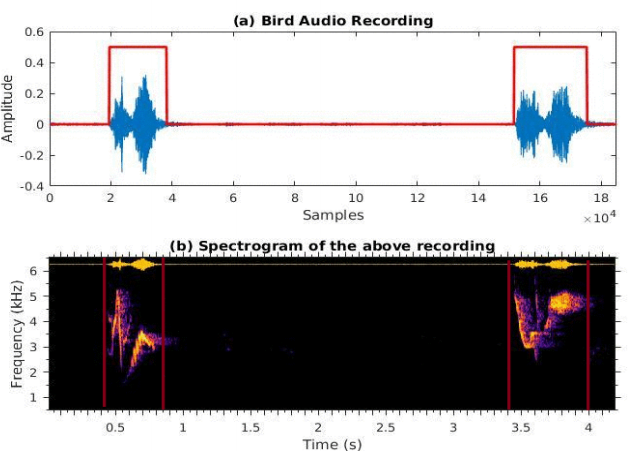
\includegraphics[width=\textwidth]{bird_spec}
\end{center}

\subsubsection{perceptrons}
\par
